\documentclass[letterpaper,11pt]{article}

\usepackage{amsmath}
\usepackage{amssymb}
\usepackage[hmargin=1.25in,vmargin=1in]{geometry}
\usepackage{booktabs}
\usepackage{graphicx}
\usepackage{hyperref}
\usepackage{lmodern}
\usepackage{microtype}

\title{Coursework 1: STAT 570}
\author{Philip Pham}
\date{\today}

\begin{document}
\maketitle

\begin{enumerate}
\item The data we analyze are from a 1970s study that investigated insurance
  redlining on $n = 47$ zipcodes. Information on who was being refused
  homeowners is not available so instead we take as response the number of FAIR
  plan policies written and renewed in Chicago by zip code over the period
  December 1977 to May 1978. The FAIR plan was offered by the city of Chicago as
  a default policy to homeowners who had been rejected by the voluntary market.
  The data we will analyze are named \texttt{chredlin} and are in the
  \texttt{faraway} package. The variable \texttt{involact} are the number of new
  FAIR plan policies and renewals per 100 housing units.

  We will consider five covariates for modeling the response: racial composition
  in percent minority (\texttt{race} $x_{i1}$), fires per 100 housing units
  (\texttt{fire} $x_{i2}$), theft per 1000 population (\texttt{theft} $x_{i3}$),
  percent of housing units built before 1939 (\texttt{age} $x_{i4}$), log
  median family income in thousands of dollars (\texttt{lincome} $x_{i5}$`),
  $i = 1,\ldots,47$.

  We will examine the model with the main effects due to race, fire, theft, age
  and $\log(\mathrm{income})$.

  We let $Y_i$ represent \texttt{involact}, and
  $x_i = \left(x_{i1}, x_{i2}, \ldots, x_{i5}\right)$, the covariates, for
  individual $i$, $i = 1,2,\ldots,47$. We fit the model
  \begin{equation}
    y_i = \beta_0 + \sum_{j=1}^5x_{ij}\beta_j + \epsilon_i
    \label{eqn:p1_model}
  \end{equation}
  for $i=1,\ldots,n$ using least squares.

  \begin{enumerate}
  \item Provide informative plots to illustrate what we might expect to learn
    from the model in Equation \ref{eqn:p1_model}.
    \label{part:p1a}

    \begin{description}
    \item[Solution:] See Figure \ref{fig:p1_pair_plots} and the corresponding
      code in
      \href{https://nbviewer.jupyter.org/github/ppham27/stat570/blob/master/hw1/chredlin\_explore.ipynb}{\texttt{chredlin\_explore.ipynb}}.

      \texttt{fire}, \texttt{race}, and \texttt{age} appear to be positively
      correlated with \texttt{involact}. \texttt{income} appears to be
      negatively correlated.

      Zipcodes in the northern \texttt{side} of Chicago have a lower minority
      population and higher income. \texttt{involact} is smaller in these
      northern zipcodes, too.
    \end{description}
  \item Give interpretations of the parameters $\beta_j$, $j = 1,\ldots,5$.
    \label{part:p1b}
    \begin{table}
      \centering
      \begin{tabular}{lrrrr}
\toprule
{} &  estimate &  std\_error &  t-statistic &   p-value \\
\midrule
(intercept) & -1.185540 &   1.100255 &    -1.077514 &  0.287550 \\
race        &  0.009502 &   0.002490 &     3.816831 &  0.000449 \\
fire        &  0.039856 &   0.008766 &     4.546588 &  0.000048 \\
theft       & -0.010295 &   0.002818 &    -3.653264 &  0.000728 \\
age         &  0.008336 &   0.002744 &     3.037749 &  0.004134 \\
log\_income  &  0.345762 &   0.400123 &     0.864137 &  0.392540 \\
\bottomrule
\end{tabular}

      \caption{The result of fitting the model described in Equation
        \ref{eqn:p1_model}. The procedure for obtaining the estimates and test
        statistics is described in Part \ref{part:p1_model}.}
      \label{tab:p1_model_parameters}
    \end{table}

    \begin{description}
    \item[Solution:] Fitting such a model, we get the estimates in Table
      \ref{tab:p1_model_parameters} for $\beta_j$.

      The percent of minorities (\texttt{race}) and frequency of fires
      (\texttt{fire}) are positively correlated with the number of FAIR plan
      policies. \texttt{involact} is the number of FAIR plans per 100 housing
      units. Thus, every percent increase in racial minorities means about 1
      FAIR plan, and for every fire per 100 housing units, there are 3 FAIR
      plans.

      \texttt{age} seems to have postive effect on \texttt{involact}, while
      \texttt{theft} has a negative effect.

      \texttt{log\_income} doesn't seem to tell us anything new: it's correlated
      with other covariates, and its effect is mainly due to chance.      
    \end{description}
    
  \item Reproduce every number in the handout using matrix and arithmetic
    operations.
    \label{part:p1_model}

    \begin{description}
    \item[Solution:] Let us assume that
      $\epsilon_i \sim \mathcal{N}\left(0, \sigma^2\right)$. The log-likelihood
      of this model is
      \begin{align}
        \sum_{i=1}^n \log\mathbb{P}\left(y_i \mid x_i, \beta, \sigma^2\right)
        &= -\frac{n}{2}\log\left(2\pi\sigma^2\right)
          - \frac{1}{2\sigma^2}\sum_{i=1}^n \left(y_i - x_i^\intercal\beta\right)^2
          \nonumber \\
        &= -\frac{n}{2}\log\left(2\pi\sigma^2\right) - \frac{1}{2\sigma^2}\left\lVert
          y - X\beta
          \right\rVert_2^2,
          \label{eqn:p1_log_likelihood}
      \end{align}
      where we $0$-index $\beta$ and the columns of $X$, so each row of $X$ is
      $x_i = \left(1, x_{i1}, x_{i2},\ldots,x_{i5}\right)$.

      \subsection*{Estimating $\hat{\beta}$}

      To maximize Equation \ref{eqn:p1_log_likelihood}, we choose $\hat{\beta}$
      such that $X\hat{\beta}$ is the projection of $y$ onto the hyperplane
      spanned by the columns of $X$. Thus, we must have that
      $X^\intercal\left(y - X\hat{\beta}\right) = 0$ since the residuals will
      orthogonal to the columns of $X$ if $X\hat{\beta}$ is the projection that
      minimizes the squared error. Solving for $\hat{\beta}$, we have that
      \begin{equation}
        \hat{\beta} = \left(X^\intercal X\right)^{-1} X^\intercal y.
        \label{eqn:p1_beta_hat}
      \end{equation}
      The results of apply Equation \ref{eqn:p1_beta_hat} can be seen in the
      first column of Table \ref{tab:p1_model_parameters}.

      \subsection*{Estimating $\hat{\sigma}^2$}

      Let us derive an unbiased estimator for residual standard error. Consider
      the residual random vector.

      \begin{equation}
        R = y - X\hat{\beta}
      \end{equation}

      As stated earlier, the residuals are orthogonal to hyperplane spanned by
      the columns of $X$, so they must lie in some orthonormal hyperplane of
      $N - p$ vectors, where $p = \dim(\beta)$. Thus, residuals are $y$
      projected down to this space.

      Let $w_1,\ldots,w_{n-p}$ be an orthonormal basis of this space. Let $W$ be
      matrix with these basis vectors as the columns.

      We have that
      \begin{align}
        R &= y - X\hat{\beta} \nonumber\\
          &= W\left(W^\intercal y\right) \nonumber\\
          &= W\left(W^\intercal\left(X\beta + \sigma\epsilon\right)\right) \nonumber\\
          &= W\left(W^\intercal X\right)\beta + \sigma W\left(W^\intercal\epsilon\right) \nonumber\\
          &= \sigma W\left(W^\intercal\epsilon\right).
      \end{align}

      Now, $W^\intercal\epsilon \sim \mathcal{N}\left(0, I_{n-p}\right)$. To see
      this, note that the $i$th entry is
      $\sum_{j=1}^n w_{ij}\epsilon_j \sim \mathcal{N}\left(0, 1\right)$, and for
      $i \neq i^\prime$,
      \begin{align*}
        \operatorname{Cov}\left(
        \left(W^\intercal\epsilon\right)_i, \left(W^\intercal\epsilon\right)_{i^\prime}\right)
        &=
          \mathbb{E}\left[
          \left(\sum_{j=1}w_{ij}\epsilon_j\right)\left(\sum_{k=1}w_{i^\prime k}\epsilon_k\right)
          \right] \\
        &= \sum_{j=1}^n\mathbb{E}\left[w_{ij}w_{i^\prime j} \epsilon_j^2\right] +
          2\sum_{j=1}^{n-1}\sum_{k=j+1}^n \mathbb{E}\left[w_{ij}w_{i^\prime k} \epsilon_j\epsilon_k\right] \\
        &= w_i^\intercal w_{i^\prime} + 2\sum_{j=1}^{n-1}\sum_{k=j+1}^n w_{ij}w_{i^\prime k}
          \mathbb{E}\left[\epsilon_j\epsilon_k\right] \\
        &= 0,
      \end{align*}
      where the first term disappears by since the two vectors are orthonormal,
      and the second term disappears because of independence of the errors.

      Thus, we have that

      \begin{equation}
        R^\intercal R
        = \sigma^2 \left(W^\intercal\epsilon\right)^\intercal W^\intercal W \left(W^\intercal\epsilon\right)
        = \sigma^2 \left(W^\intercal\epsilon\right)^\intercal\left(W^\intercal\epsilon\right)
        \sim \sigma^2 \chi^2_{n-p}.
        \label{eqn:p1_residual_distribution}
      \end{equation}

      Finally, we have that

      \begin{equation*}
        \mathbb{E}\left[R^\intercal R\right] = \sigma^2\left(n - p\right)
        \Rightarrow
        \mathbb{E}\left[\frac{\sum_{i=1}^n \left(y - X\hat{\beta}\right)^2}{n-p}\right] = \sigma^2.
      \end{equation*}

      Our consistent estimator is

      \begin{equation}
        \hat{\sigma}^2 = \frac{\sum_{i=1}^n \left(y - X\hat{\beta}\right)^2}{n-p}.
        \label{eqn:p1_sample_variance}
      \end{equation}

      Applying Equation \ref{eqn:p1_sample_variance}, we obtain
      \boxed{\hat{\sigma} = \input{p1_residual_standard_error.txt}\unskip.}

      \subsection*{Hypothesis Testing}

      We can rewrite $y$ as $y = X\beta + \sigma \epsilon$, where each element
      of $\epsilon$ is drawn from $\mathcal{N}\left(0, 1\right)$. Substituting,
      we have that
      \begin{align}
        \hat{\beta}
        &= \left(X^\intercal X\right)^{-1}X^\intercal\left(X\beta + \sigma\epsilon\right) \nonumber\\
        &= \beta + \sigma\left(X^\intercal X\right)^{-1}X^\intercal \epsilon.
          \label{eqn:p1_beta_hat_distribution}
      \end{align}

      Thus, $\hat{\beta}_j \sim \mathcal{N}\left(\beta_j, \sigma^2\left(X^\intercal X\right)^{-1}_{jj}\right)$.

      This gives us that
      \begin{equation*}
        \frac{\hat{\beta}_j - \beta_j}{\sqrt{\sigma^2\left(X^\intercal X\right)^{-1}_{jj}}} \sim
        \mathcal{N}\left(0, 1\right).
      \end{equation*}

      From Equations \ref{eqn:p1_residual_distribution} and \ref{eqn:p1_sample_variance},
      \begin{equation}
        (n - p)\frac{\hat{\sigma}^2}{\sigma^2} \sim \chi^2_{n-p}.
      \end{equation}

      $\hat{\beta}$ and $\hat{\sigma}^2$ are independent by
      \href{https://en.wikipedia.org/wiki/Basu\%27s_theorem}{Basu's theorem}:
      $\hat{\sigma}^2$ is an ancillary statistic that does not depend on the
      model parameters, $\beta$. Thus, we have that
      \begin{equation}
        \left.
          \frac{\hat{\beta}_j - \beta_j}{\sqrt{\sigma^2\left(X^\intercal X\right)^{-1}_{jj}}}
          \middle/
          \sqrt{\frac{(n - p)\frac{\hat{\sigma}^2}{\sigma^2}}{n-p}}
        \right. 
        = \frac{\hat{\beta}_j - \beta_j}{\sqrt{\hat{\sigma}^2\left(X^\intercal X\right)^{-1}_{jj}}}
        \sim t_{n-p}.
        \label{eqn:p1_beta_hat_j_distribution}
      \end{equation}

      That is, we have $t$ distribution with $n - p$ degrees of freedom. The
      denominator of Equation \ref{eqn:p1_beta_hat_j_distribution} gives the
      second column of Table \ref{tab:p1_model_parameters}.

      For each $\beta_j$, our null hypothesis is $H_0: \beta_j = 0$. Thus, our
      $t$-test statistic is obtain from substituting $\beta_j$ into Equation
      \ref{eqn:p1_beta_hat_j_distribution},
      \begin{equation*}
        \hat{t}_j = \frac{\hat{\beta}_j}{\sqrt{\hat{\sigma}^2\left(X^\intercal X\right)^{-1}_{jj}}},
      \end{equation*}
      which gives us the third column of Table \ref{tab:p1_model_parameters}.

      The fourth column is the probability of obtaining evidence that
      contradicts the null hypothesis at least as much. Let $F^{-1}_{t_{n-p}}$
      be the inverse cumulative distribution function. The $p$-value is
      \begin{equation*}
        \mathbb{P}\left(
          \left\lvert T_{n - p}\right\rvert \geq
          \left\lvert \hat{t}_j\right\rvert
          \mid
          \hat{t}_j
        \right) = 
        2\left(1 - F^{-1}_{n - p}\left(\left\lvert\hat{t}_j\right\rvert\right)\right).
      \end{equation*}

      These calculations are carried out in
      \href{https://nbviewer.jupyter.org/github/ppham27/stat570/blob/master/hw1/chredlin\_model.ipynb}{\texttt{chredlin\_explore.ipynb}}.
    \end{description}
    
  \item What assumptions are valid for:
    \begin{enumerate}
    \item An unbiased estimate of $\beta_j$, $j = 1,\ldots,5$.
      \label{part:p1di}
        
      \begin{description}
      \item[Solution:] From Equation \ref{eqn:p1_beta_hat_distribution}, we have
        that
        \begin{equation}
          \mathbb{E}\left[\hat{\beta}\right]
          =
          \beta + \left(X^\intercal X\right)^{-1}X^\intercal \mathbb{E}\left[\epsilon\right]
        \end{equation}
        since expectation is a linear operator. In our previous calcuations, we
        assumed that the $\epsilon_i$ were independent and normally distributed.

        It's sufficient, however, that
        $\boxed{\mathbb{E}\left[\epsilon\right] = \mathbf{0}.}$ Then, we'll have
        \begin{equation*}
          \operatorname{bias}\left(\hat{\beta}\right) =
          \mathbb{E}\left[\hat{\beta}\right] - \beta
          = \beta - \beta = 0.
        \end{equation*}
      \end{description}
    \item An accurate estimate of the standard error of $\hat{\beta}_j$,
      $j = 1,\ldots,5$.

      \begin{description}
      \item[Solution:] From Equation \ref{eqn:p1_beta_hat_distribution}, we can
        estimate the standard error exactly if $\sigma^2$ is known. For
        $\hat{\beta}_j$, we get $\sigma\sqrt{\left(X^\intercal X\right)_{jj}^{-1}}$.

        When $\sigma^2$ is unknown, but our errors are still independent and
        normally distributed, we apply Equation
        \ref{eqn:p1_beta_hat_j_distribution}. Since $\hat{\beta}_j$ has Student's
        $t$-distribution, we can estimate the standard error for $\hat{\beta}_j$
        with $\sqrt{\hat{\sigma}^2\left(X^\intercal X\right)_{jj}^{-1}}$.

        If our errors are not normally distributed, our estimate is only
        accurate if the number of observations is large, and our errors have a
        distribution that converges to a normal distribution.
      \end{description}
    \item Accurate coverage probabilities for $100\left(1 - \alpha\right)\%$
      confidence intervals of the form
      \begin{equation}
        \hat{\beta}_j \pm \sqrt{\hat{\sigma}_j^2}z_{1-\alpha/2},
        \label{eqn:p1_confidence_interval_normal}
      \end{equation}
      where $z_{1-\alpha/2}$ represents the $\left(1-\alpha/2\right)$ quantile
      of an $\mathcal{N}\left(0, 1\right)$ random variable, and
      $\hat{\sigma}_j^2 = \hat{\sigma}^2\left(X^\intercal X\right)_{jj}^{-1}$.

      \begin{description}
      \item[Solution:] Firstly, the assumptions from the previous part must hold
        for $\hat{\sigma}_j^2$ to be meaningful.

        From Equation \ref{eqn:p1_beta_hat_j_distribution}, $\hat{\sigma}_j^2$
        has Student's $t$-distribution, so the normal approximation for the the
        confidence interval (Equation \ref{eqn:p1_confidence_interval_normal})
        only holds when $n$ is large.
      \end{description}
            
    \item Accurate coverage probabilities for $100\left(1 - \alpha\right)\%$
      confidence intervals of the form

      \begin{equation}
        \hat{\beta}_j \pm \sqrt{\hat{\sigma}_j^2}t_{n-p}\left(1-\alpha/2\right),
        \label{eqn:p1_confidence_interval_t}
      \end{equation}
      where $p = \dim\left(\beta\right)$ and $t_{n-p}\left(1-\alpha/2\right)$
      represents the $\left(1-\alpha/2\right)$ quantile of standard Student's
      $t$ random variable with $n - p$ degrees of freedom.

      \begin{description}
      \item[Solution:] Equation \ref{eqn:p1_beta_hat_j_distribution} shows that
        this is exactly the correct distribution when the $\epsilon_i$ are
        independent and identically distributed as normal random variables with
        mean zero.

        It may still prove to be an accurate confidence interval if the errors
        have distributions that are well-approximated by the normal
        distribution and the number of observations is large.
      \end{description}
    \item An accurate prediction for an \emph{observed} outcome at $x_0$.
      
      \begin{description}
      \item[Solution:] Suppose we were to observe
        $\left(x_0, y_0 = x_0^\intercal\beta + \epsilon_0\right)$. Let our
        prediction be $\hat{y}_0 = x_0^\intercal\hat{\beta}$. If the conditions
        in Part \ref{part:p1di} are satisfied, the error has mean zero, and our
        estimate for $\hat{\beta}$ is unbiased, so
        \begin{equation*}
          \mathbb{E}\left[y_0\right]
          = x_0^\intercal\beta
          = \mathbb{E}\left[\hat{y}_0\right].
        \end{equation*}
        
        We want to compare our prediction with $\hat{y}_0$ with some
        hypothetical observed response $y_0$. We'll call our prediction
        accurate within $\delta > 0$ if
        \begin{equation*}
          \hat{y}_0 - \delta \leq y_0 \leq \hat{y}_0 + \delta.
        \end{equation*}

        We want the probability of this event to be high, so we'll say accurate
        within $\delta$ at confidence level $1 - \alpha$ if
        \begin{equation*}
          \mathbb{P}\left(\hat{y}_0 - \delta \leq y_0 \leq \hat{y}_0 + \delta\right)
          = \mathbb{P}\left(-\delta \leq y_0 - \hat{y}_0 \leq \delta\right)
          \geq 1 - \alpha.
        \end{equation*}
        Our prediction is accurate if for small $\alpha$, we have small
        $\delta$.

        If we assume normality, we can calculate the minimum $\delta$ for a
        specific $\alpha$, which we'll denote $\delta_\alpha$.

        Since $\hat{\beta}$ satisfies
        $\left(X^\intercal X\right)\hat{\beta} = X^\intercal y$, we have that
        the intercept estimate is
        \begin{equation}
          \hat{\beta}_0 = \bar{y} - \sum_{j=1}^p \hat{\beta}_j \bar{X}_{:,j}.
        \end{equation}

        Consider trying to predict $\hat{y} = x^\intercal\hat{\beta}$ for some
        $x$. We have that
        \begin{equation}
          \hat{y} = \bar{y} + \sum_{j=1}^p \left(x_i - \bar{X}_{:,j}\right)\hat{\beta}_j,
        \end{equation}
        so the variance of the prediction increases with values far from data.

        Let $\bar{X}$ be the vector of column-wise means of $X$. Since
        $\bar{\epsilon}$ is an ancillary statistic, this can also be written as

        \begin{equation}
          \hat{y} \mid x \sim \mathcal{N}\left(
            x^\intercal \beta,
            \sigma^2 \left(
              \frac{1}{n} +
              \left(x - \bar{X}\right)^\intercal
              \left(X^\intercal X\right)^{-1}
              \left(x - \bar{X}\right)
            \right)
          \right).
        \end{equation}

        Using the same method as in deriving Equation
        \ref{eqn:p1_beta_hat_j_distribution}, if we replace $\beta$ with
        $\hat{\beta}$ and $\sigma^2$ with $\hat{\sigma}^2$, we have
        \begin{equation}
          \frac{\hat{y} - x^\intercal\hat{\beta}}{
            \sqrt{\hat{\sigma}^2\left(\frac{1}{n} +
              \left(x - \bar{X}\right)^\intercal
              \left(X^\intercal X\right)^{-1}
              \left(x - \bar{X}\right)\right)}}
          \sim t_{n-p}.
          \label{eqn:p1_response_confidence_interval}
        \end{equation}

        Noting that
        $y_0 \sim \mathcal{N}\left(x_0^\intercal\beta, \sigma^2\right)$, we can
        apply Equation \ref{eqn:p1_response_confidence_interval} to
        $\left(x_0, y_0\right)$, which gives us
        \begin{equation*}
          \boxed{
            \delta_\alpha
            =
            t_{n-p}\left(1 - \alpha/2\right)
            \sqrt{\hat{\sigma}^2\left(
                1 + \frac{1}{n} +
                \left(x_0 - \bar{X}\right)^\intercal
                \left(X^\intercal X\right)^{-1}
                \left(x_0 - \bar{X}\right)
              \right).
            }
          }
        \end{equation*}

        Thus, our predictions will always have standard error of at least
        $\sigma$, but they will be more accurate when $x_0$ is close to
        $\bar{X}$.
      \end{description}
    \end{enumerate}
  \item Summarize the relationship between $y$, and $x_1$, $x_2$, $x_3$, $x_4$,
    $x_5$, fitting any other models that you see fit to.

    \begin{description}
    \item[Solution:] The relationship between $y$ and the covariates was
      described in Parts \ref{part:p1a} and \ref{part:p1b}.

      Particularly, we see \texttt{income} does not explain much about
      \texttt{involact} due to multicollinearity: it is correlated with
      \texttt{race} and \texttt{fire}.

      Removing \texttt{log\_income} from the model gives us the model parameters
      in Table \ref{tab:p1_model_parameters_custom}. The residual standard error
      for this model was \input{p1_residual_standard_error_custom.txt}\unskip,
      which is actually ever so slightly smaller than the model that includes
      income.

      \begin{table}
        \centering
        \begin{tabular}{lrrrr}
\toprule
{} &  estimate &  std\_error &  t-statistic &   p-value \\
\midrule
(intercept) & -0.243118 &   0.145054 &    -1.676054 &  0.101158 \\
race        &  0.008104 &   0.001886 &     4.296913 &  0.000100 \\
fire        &  0.036646 &   0.007916 &     4.629173 &  0.000035 \\
theft       & -0.009592 &   0.002690 &    -3.565847 &  0.000921 \\
age         &  0.007210 &   0.002408 &     2.994369 &  0.004595 \\
\bottomrule
\end{tabular}

        \caption{The result of fitting a model without considering income.}
        \label{tab:p1_model_parameters_custom}
      \end{table}

      I tried adding an indicator for \texttt{side} but it suffers from the same
      issue as \texttt{income}: its effect is already explained by the other
      covariates.
    \end{description}
  \end{enumerate}

  \pagebreak
\item Consider the following distributions:
  \begin{description}
  \item[Poisson:] \begin{equation}
      p\left(y \mid \mu\right) = \frac{\exp\left(-\mu\right)\mu^y}{y!},
      \label{eqn:p2_poisson}
    \end{equation}
    for $y = 0,1,2,\ldots$.
    
  \item[Gamma:] \begin{equation}
      p\left(y \mid \alpha, \beta\right) =
      \frac{\beta^\alpha}{\Gamma(\alpha)}y^{\alpha - 1}\exp(-\beta y)
      \label{eqn:p2_gamma}
    \end{equation}
    for $y > 0$ and with $\alpha$ known.
    
  \item[Inverse Gaussian:]
    \begin{equation*}
      p\left(y \mid \mu, \delta\right) =
      \left(\frac{\delta}{2\pi y^3}\right)^{1/2}
      \exp\left[
        \frac{-\delta\left(y-\mu\right)^2}{2\mu^2y}
      \right]
      \label{eqn:p2_inverse_gaussian}
    \end{equation*}
    for $y > 0$ and $\delta$ known.

  \end{description}

  A distribution is said to be a member of the one parameter exponential family
  of distributions if it can be written as
  \begin{equation}
    p\left(y \mid \eta_1,\eta_2\right) = h(y)\exp\left[
      \eta_1y + \eta_2T_2(y) - A\left(\eta_1,\eta_2\right)
    \right],
    \label{eqn:p2_exponential}    
  \end{equation}
  where $\eta_2$ is known.
  
  \begin{enumerate}
  \item Show that each of the above distributions is a member of the exponential
    family and identify $\eta_1$, $\eta_2$, $T_2(y)$,
    $A\left(\eta_1,\eta_2\right)$, and $h(y)$.
    \label{part:p2a}
    \begin{description}
    \item[Solution:] For each distribution, we can do some algebra.
      
      \begin{description}
      \item[Poisson:] We can rewrite Equation \ref{eqn:p2_poisson} as Equation
        \ref{eqn:p2_exponential}, where
        \begin{align*}
          \eta_1 &= \log\mu \\
          \eta_2 &= 0 \\
          T_2(y) &= 0 \\          
          A\left(\eta_1,\eta_2\right) &= \exp(\eta_1) \\
          h(y) &= \frac{1}{y!}.
        \end{align*}
      \item[Gamma:] We can rewrite Equation \ref{eqn:p2_gamma} as Equation
        \ref{eqn:p2_exponential}, where
        \begin{align*}
          \eta_1 &= -\beta \\
          \eta_2 &= \alpha - 1 \\
          T_2(y) &= \log(y) \\
          A\left(\eta_1,\eta_2\right)
                 &=-\left(\eta_2 + 1\right)\log\left(-\eta_1\right) +
                   \log\Gamma\left(\eta_2 + 1\right)\\
          h(y) &= 1.
        \end{align*}
      \item[Inverse Gaussian:] We can rewrite Equation \ref{eqn:p2_inverse_gaussian} as
        Equation \ref{eqn:p2_exponential}, where
        \begin{align*}
          \eta_1 &= -\frac{\delta}{2\mu^2} \\
          \eta_2 &= -\frac{\delta}{2} \\
          T(y) &= \frac{1}{y} \\
          A\left(\eta_1,\eta_2\right)
                 &= -2\sqrt{\eta_1\eta_2} -
                   \frac{1}{2}\log\left(-2\eta_2\right) \\
          h(y) &= \frac{1}{\sqrt{2\pi y^3}}.
        \end{align*}
      \end{description}      
    \end{description}
  \item Identify $\mathbb{E}\left[Y \mid \theta\right]$ and
    $\operatorname{Var}\left(Y \mid \theta\right)$.
    \begin{description}
    \item[Solution:] We can derive a general formula for computing the mean and
      variance from Equation \ref{eqn:p2_exponential}.

      The log-likelihood function is
      \begin{equation}
        l\left(
          \eta_1, \eta_2
        \right) =
        \log h(y) + \eta_1y + \eta_2 T_2(y) - A\left(\eta_1,\eta_2\right).
      \end{equation}

      If $\eta_2$ is known, the score function is
      \begin{equation}
        S\left(\eta_1, \eta_2\right) = \frac{\partial l\left(\eta_1,\eta_2\right)}{\partial \eta_1}
        =
        y - \frac{\partial A\left(\eta_1,\eta_2\right)}{\partial \eta_1}.
      \end{equation}

      The expectation of the score is $0$, so
      \begin{equation}
        \boxed{\mathbb{E}\left[y \mid \eta_1, \eta_2\right] =
        \frac{\partial A\left(\eta_1,\eta_2\right)}{\partial \eta_1}.}
        \label{eqn:p2_score_mean}
      \end{equation}

      The variance of the score is Fisher information, so
      \begin{align}
        \mathcal{I}\left(\eta_1, \eta_2\right)
        &=
        \operatorname{Var}\left(
        S\left(\eta_1, \eta_2\right)
          \right) \nonumber\\
        &= \mathbb{E}\left[
          \left(y -
          \frac{\partial A\left(\eta_1,\eta_2\right)}{\partial \eta_1}
          \right)^2
          \mid
          \eta_1, \eta_2
          \right]\nonumber\\
        &= \operatorname{Var}\left(y \mid \eta_1, \eta_2\right)
          \label{eqn:p2_fisher_variance}
      \end{align}
      by Equation \ref{eqn:p2_score_mean}
      and using that the mean of the score function is $0$.

      An alternative definition of the Fisher information is the expected value
      of the observed information:
      \begin{equation}
        \mathcal{I}\left(\eta_1, \eta_2\right) =
        - \frac{\partial^2 l\left(\eta_1,\eta_2\right)}{\partial\eta_1^2}
        = \frac{\partial^2 A\left(\eta_1,\eta_2\right)}{\partial\eta_1^2}.
        \label{eqn:p2_fisher_expectation}
      \end{equation}

      Combining Equations \ref{eqn:p2_fisher_variance} and
      \ref{eqn:p2_fisher_expectation}, we obtain
      \begin{equation}
        \boxed{
          \operatorname{Var}\left(y \mid \eta_1, \eta_2\right)
          =
          \frac{\partial^2 A\left(\eta_1,\eta_2\right)}{\partial\eta_1^2}.
        }
        \label{eqn:p2_score_variance}
      \end{equation}

      We can now apply Equations \ref{eqn:p2_score_mean} and
      \ref{eqn:p2_score_variance} to our the results from Part \ref{part:p2a}.
      \begin{description}
      \item[Poisson:]
        \begin{align*}
          \mathbb{E}\left[y \mid \eta_1, \eta_2\right]
          &= \exp\left(\eta_1\right) = \mu \\
          \operatorname{Var}\left(y \mid \eta_1, \eta_2\right)
          &= \exp\left(\eta_1\right) = \mu.
        \end{align*}
      \item[Gamma:]
        \begin{align*}
          \mathbb{E}\left[y \mid \eta_1, \eta_2\right]
          &= -\frac{\eta_2 + 1}{\eta_1} = \frac{\alpha}{\beta} \\
          \operatorname{Var}\left(y \mid \eta_1, \eta_2\right)
          &= \frac{\eta_2 + 1}{\eta_1^2} = \frac{\alpha}{\beta^2}.
        \end{align*}
      \item[Inverse Gaussian:]
        \begin{align*}
          \mathbb{E}\left[y \mid \eta_1, \eta_2\right]
          &= \sqrt{\frac{\eta_2}{\eta_1}} = \mu \\
          \operatorname{Var}\left(y \mid \eta_1, \eta_2\right)
          &= \frac{1}{2}\sqrt{\frac{\eta_2}{\eta_1^3}} = \frac{\mu^3}{\delta}.
        \end{align*}
      \end{description}
    \end{description}

  \item The canonical link function is such that $g(\mu) = \eta_1$. Determine the
    canonical link for each distribution.
    \begin{description}
    \item[Solution:] We can use the results from Part \ref{part:p2a}.
      \begin{description}
      \item[Poisson:] $\displaystyle g(\mu) = \exp(\mu)$.
      \item[Gamma:] $\displaystyle g(\mu) = -\frac{\alpha}{\mu} \propto \mu^{-1}$,
        where $\alpha$ is known.
      \item[Inverse Gaussian:]
        $\displaystyle g(\mu) = -\frac{\delta}{2\mu^2} \propto \mu^{-2}$, where $\delta$ is
        known.
      \end{description}
    \end{description}
  \end{enumerate}
\end{enumerate}

\begin{figure}
  \centering
  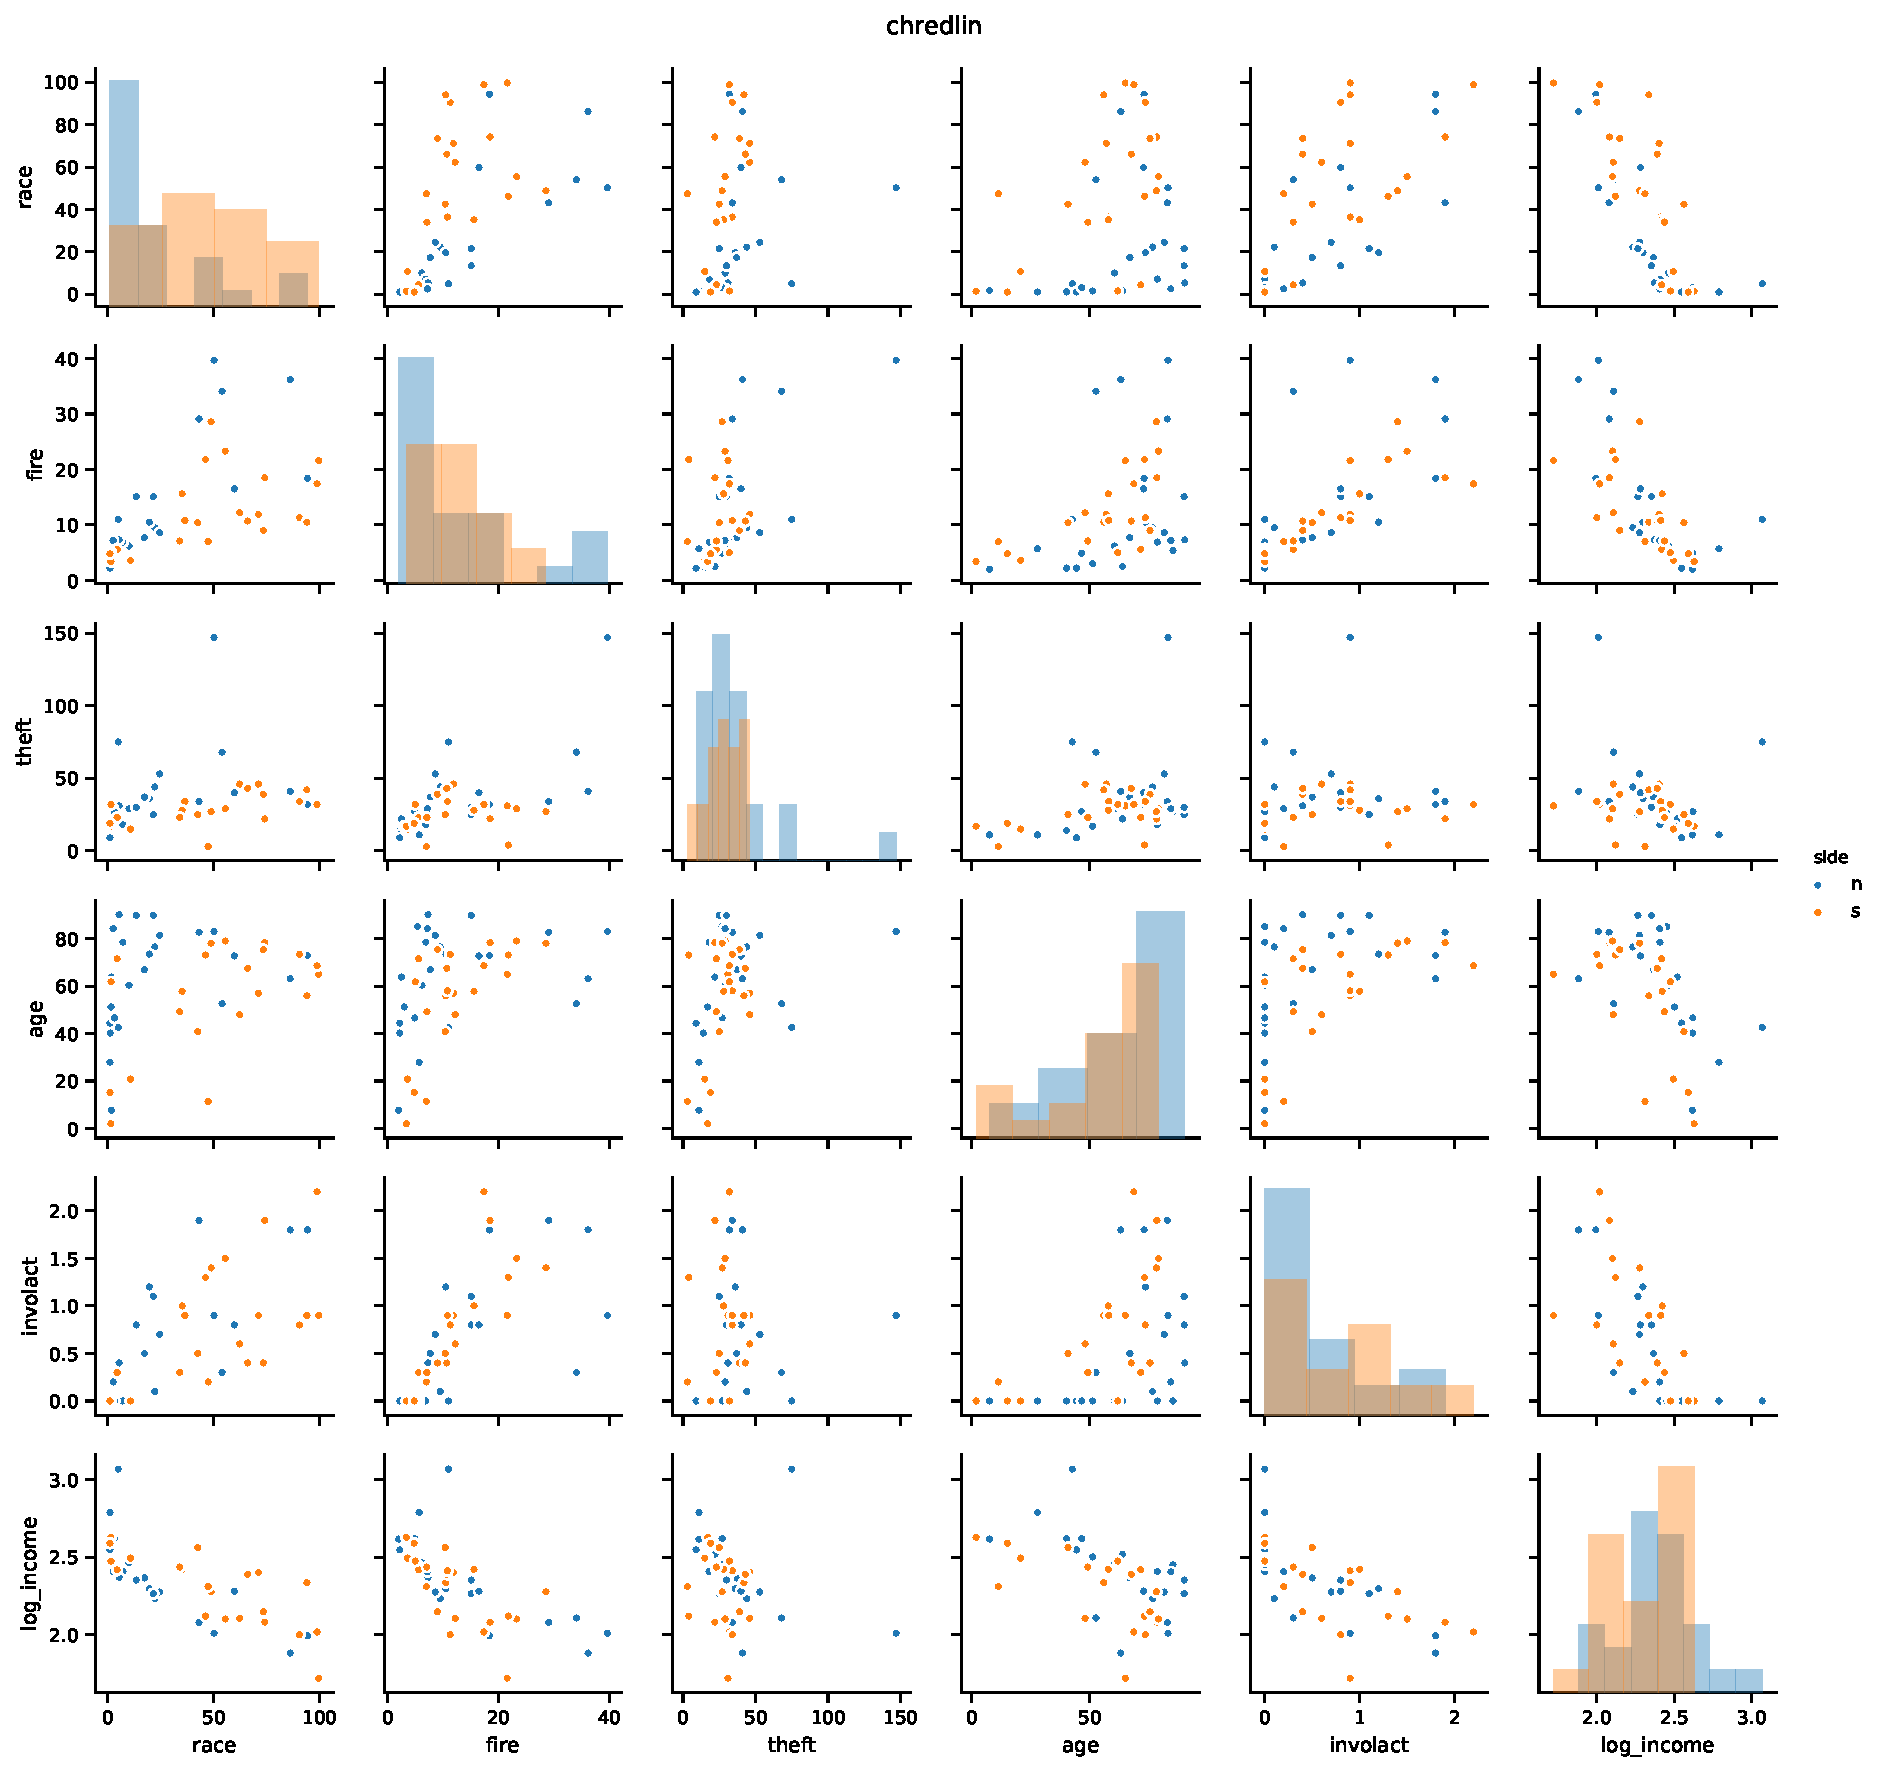
\includegraphics[width=\textwidth]{p1_pair_plots.pdf}
  \caption{The empirical univariate and joint distributions for the
    \texttt{chredlin} dataset.}
  \label{fig:p1_pair_plots}
\end{figure}

\end{document}

